
\begin{figure}[bt]
\centerline{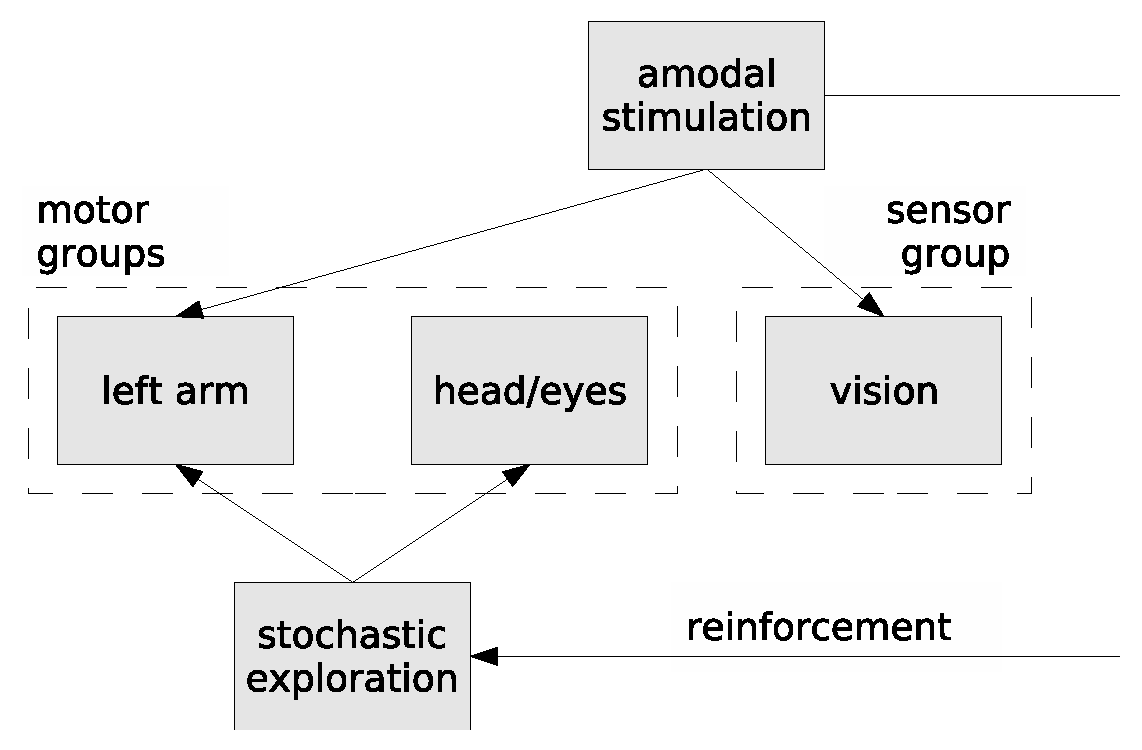
\includegraphics[height=6cm]{images/amodal-modules}}
\caption {
%
\label{fig:amodal-module-vision}
%
The system for stochastic exploration and amodal stimulation.
Exploration exercises a set of motor groups, moving them
to random locations within their nominal ranges.
Amodal stimulation modulates the state of a motor group
in a rhythmic fashion, and looks for signs of that rhythm 
showing up in a sensor group. If the amodal signal does in
fact get transmitted, a reinforcement signal is sent to the
exploration model, biasing further exploration towards the
current configuration of the motor groups.
%
The specific scenario shown here is for visual hand/arm coordination.
The state of the head and arm are explored, while watching for
an amodal connection between the arm and vision.
%
}
\end{figure}

\section{Stochastic exploration and amodal stimulation}

We have previously investigated methods for learning certain motor
skills, such as visually-guided reaching.  As part of the CONTACT
project, UGDIST is considering whether there are mechanisms for
learning such skills that are applicable to both speech and
manipulation.
%
This work revisits themes already examined, but under a more general
framework.

Figure~\ref{fig:amodal-module-vision} shows a crude but general system
for learning certain motor-sensor mappings.  We assume that the
learning problem will be posed as follows: given a collection of motor
groups and sensor groups, and a particular feature derived from the
sensed data, find a configuration of the motor groups such that local
changes in that configuration lead to systematic changes in the
derived feature.

More formally, suppose we have motor control variables
$m=(m_1,m_2,...,m_N)$ and sensor variables $s=(s_1,s_2,...,s_n)$.
Suppose we have some chosen feature of interest $f(s)$.  We know that
$s$ is a function of both $m$ and a set of environmental variables
representing all other influences and state, $e=(e_1,e_2,...)$.
We are interested in how $f$ changes with $m$:

\begin{equation}
\nabla f  = \left(\frac{\partial f}{\partial m_1 }, \frac{\partial f}{\partial m_2 }, \dots,  \frac{\partial f}{\partial m_N }  \right)
\end{equation}

We would like to maximize $|\nabla{}f|$.  We estimate this value
directly through measurement by systematically perturbing $m$ and
measuring $f$.
%
In fact, we really are only concerned with making $|\nabla{}f|$ 
non-zero, since it is quite possible that in much of the motor space 
changes in $m$ have completely no impact on $f$.
%
In that case, we can measure the change in a random motor 
direction $\Delta{}m=(\Delta{}m_1,\Delta{}m_2,...,\Delta{}m_N)$.
%
Unless we are unlucky enough to pick a direction orthogonal to 
the gradient, we should see some change in $f$.

However, as we were perturbing $m$, other environmental variables
may also have been changing, causing arbitrary effects on $f$.
We can make this less problematic by simply repeating our perturbation
rhythmically and seeing if the behavior on $f$ seems truly
systematic.


***

Implemented motor ``babble'' that uses step-wise stochastic search of
the control knobs of a motor system, ``twiddling'' them in a rhythmic
fashion.

Then looks for a ``resonance'' in a specified sensed value
(e.g. visual motion, or clear pitch).  This can be very selective to
the rhythm - helps discount unrelated events.

Gives automatic method for finding configuration of motor system that
produces desired result.


\begin{figure}[p]
\centerline{\includegraphics[width=\textwidth]{images/find-arm}}
\caption{
%
A simulated robot, performing motor exploration on its
head/eyes and left arm.  The head, eyes, and arms move around randomly
within their range of movement.
%
A periodic ``shaking'' movement of the arm is made about its
current position, and the effect of this movement is searched 
for visually.
%
When resonance occurs, the configution of head/eyes and left arm
is reinforced so that the robot is more likely to return to that
configuration.
%
This is why 
in early snapshots (top) the robot is unlikely to be looking at 
its arm, and in later snapshots (bottom) the robot is looking at
its arm more often than not.
%
}
\end{figure}

Why?

Want a way of expressing capabilities (such as "bring hand in front of head") in a robust form.

Does NOT assume a tabula rasa - in fact, there is at least as much information involved in exploration (expressing the motor groups to use, their scales, and what sensory cue to monitor) as there would be in just giving numerical pose information.

The difference is robustness to the details of the hand and the head; e.g. could use mirror.

Limitations?

Such stochastic search is very dumb.

Once an initial point of contact has been found, tracking methods would be more efficient for exploring a region of motor space.

Shaking is just one of several amodal cues that could be used (and not a very realistic one)

xref?

Could automate motor space classification examples: gesture recognition, speech recognition

Would have to be a lot simpler than offline, human-mediated work of course.


\subsection{Towards meaning}

The richer the robot's "internal life" is, the more interesting kinds
of "meanings" there can be in its world

- Continuous, broad, shared, structured experience

- Meaning as a process, not a label

Off-line data collection, segmentation, labelling, training of
classifiers, etc work, but restrict the potential semantic universe of
the robot.

For Year 3, online behaviors would be useful.

